\documentclass{article}
\usepackage[margin=0.8in]{geometry}
\usepackage{amsmath}
\usepackage{amssymb}
\usepackage{graphicx}
\usepackage{float}

\title{Mini-report for Programming Assignment 1: Question 4}
\author{Vishwak S \\
\texttt{CS15BTECH11043}}
\date{}

\begin{document}
\maketitle
\section*{Dataset choices}
\begin{itemize}
\item The missing values in the dataset were replaced by \(-1\).
\item The categorical data were converted into ordinals based on the order specified in the \texttt{README} file. 
\item After the conversion of all values: the dataset was normalized to \(\mu= 0\) and \(\sigma=1\) to ensure better spread of positive and negative values.
\end{itemize}

\section*{Best Value for Hyperparameters for the \\
Gaussian and Polynomial kernels}
\begin{flushleft}
I conducted 50 experiments for finding a sub-optimal hyperparameter \(\sigma\) for the Gaussian Kernel and 10 experiments for finding a sub-optimal hyperparameter \(q\) for the Polynomial kernel. The experiments were performed using grid-search with \(q \in \{1, 2, \ldots, 10\}\) and \(\sigma \in \{0.1, 0.2, 0.3, \ldots, 5\}\). Below are the graphs of variation of train and validation accuracies with the hyperparameters for both kernels.

\begin{figure}[H]
\begin{minipage}{0.45\linewidth}
\centering
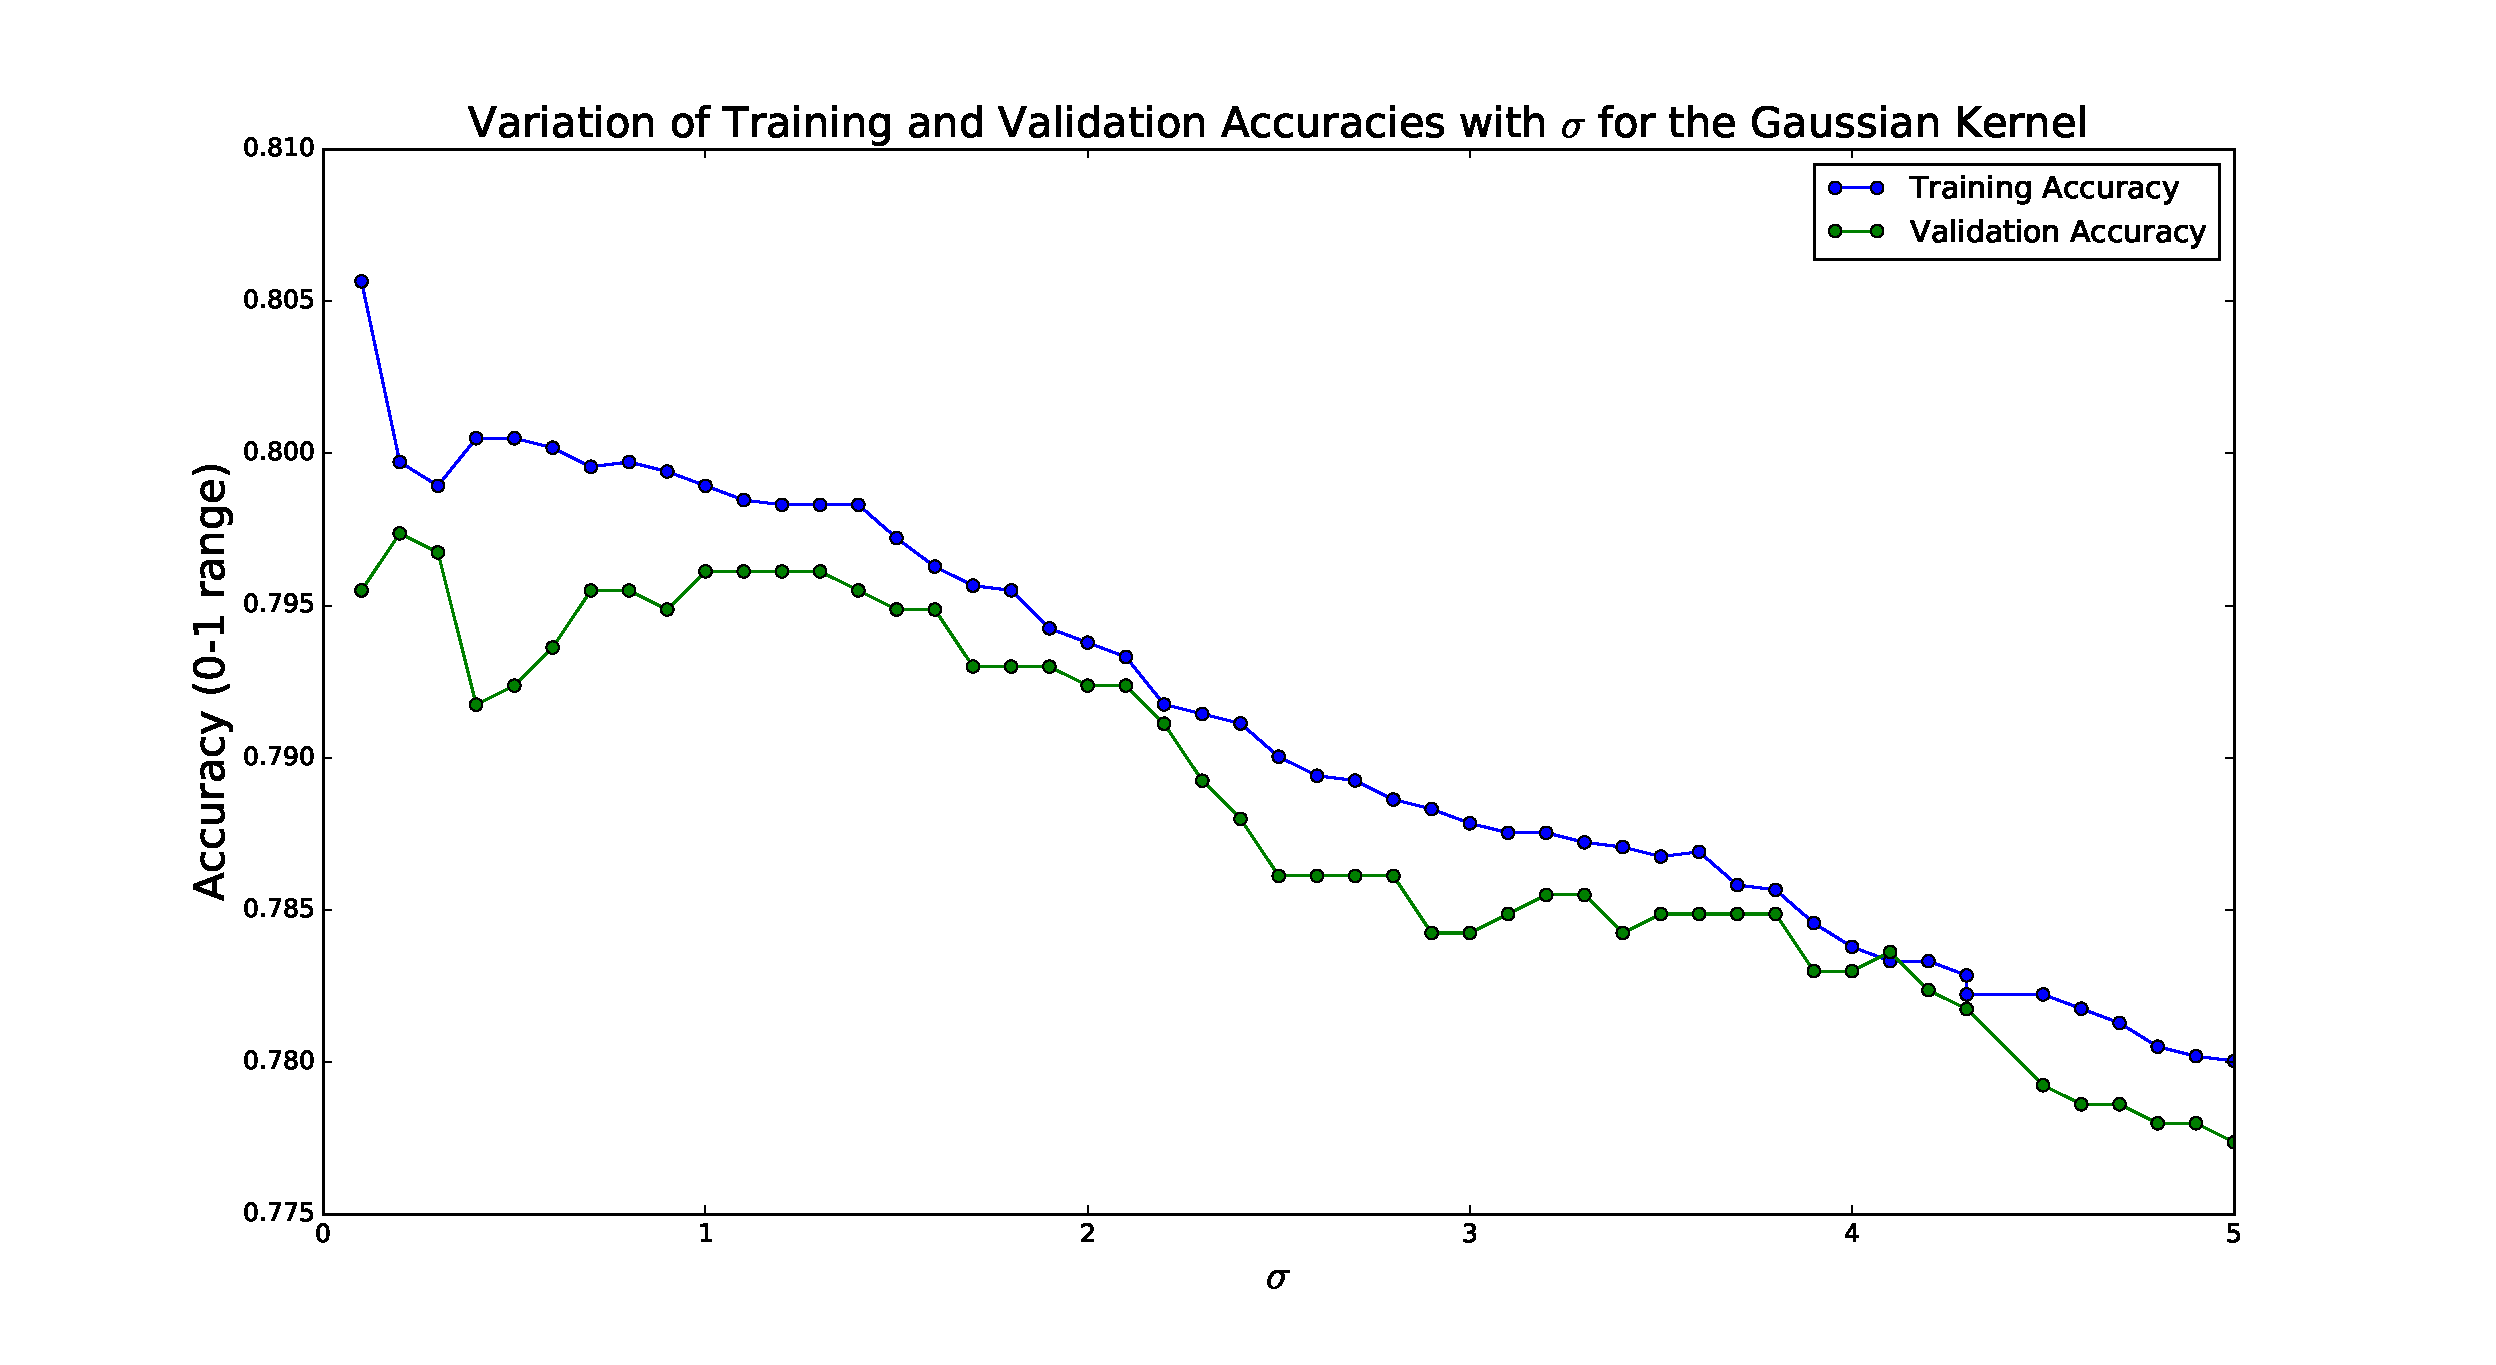
\includegraphics[width=0.95\textwidth]{./images/gaussian.eps}
\end{minipage}
\hfill
\begin{minipage}{0.45\linewidth}
\centering
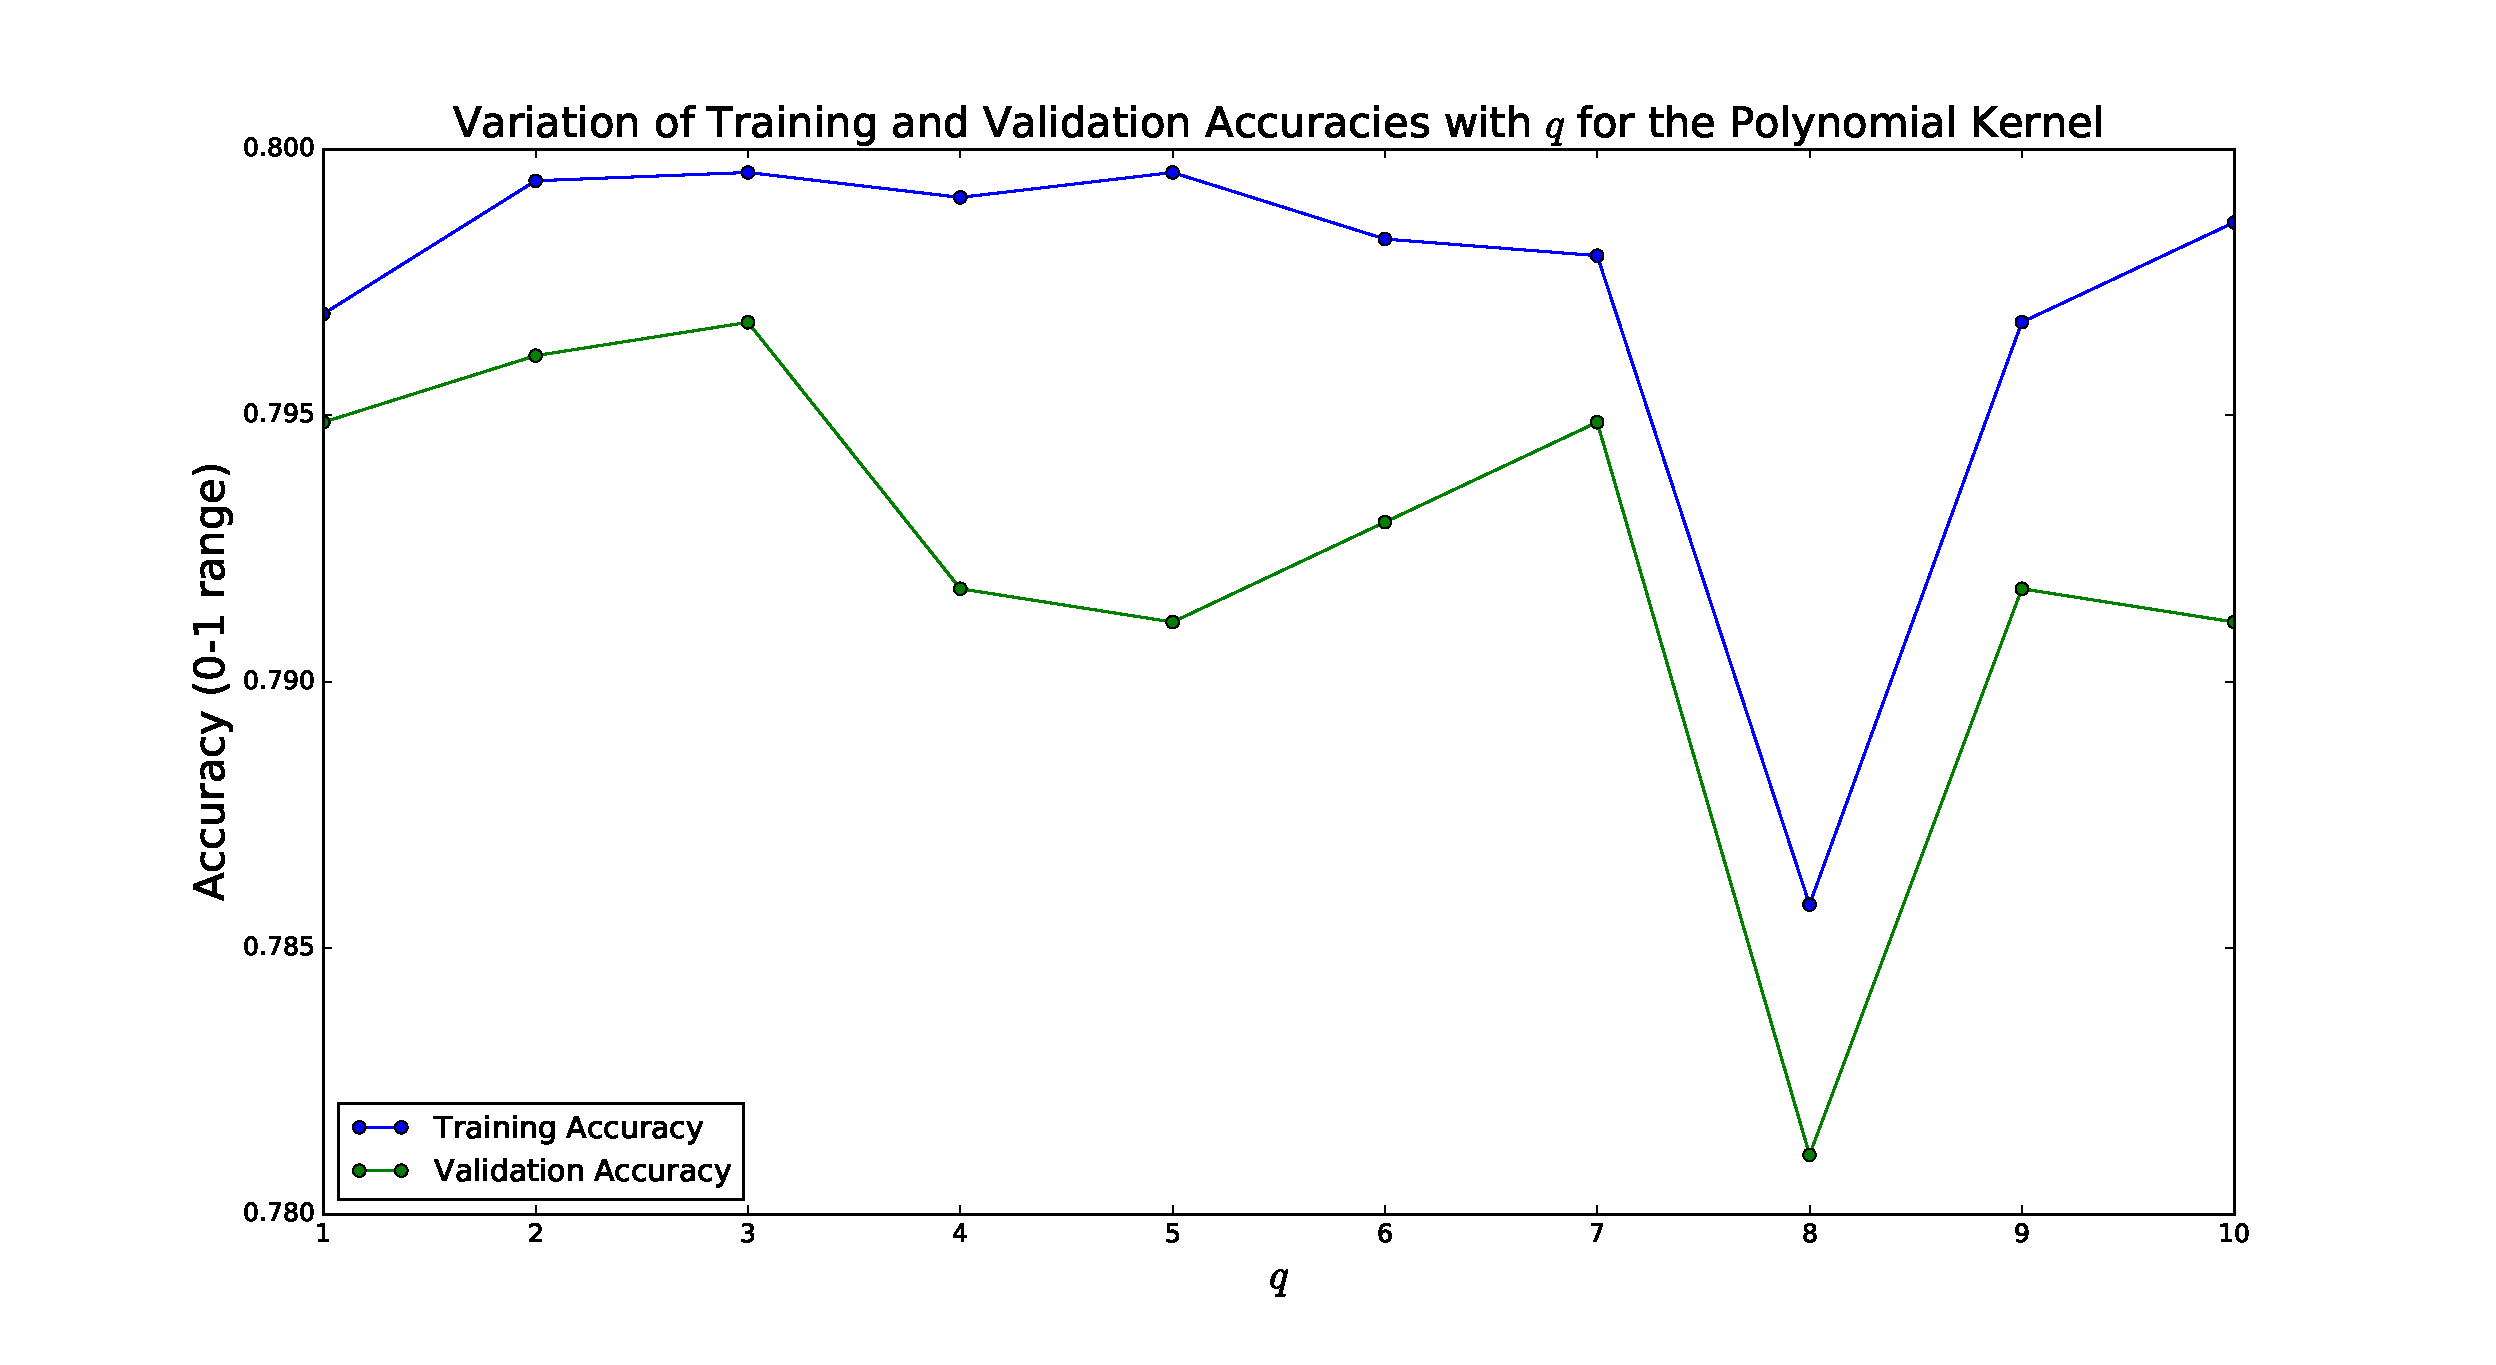
\includegraphics[width=0.95\textwidth]{./images/polynomial.eps}
\end{minipage}
\end{figure}
\end{flushleft}

\section*{Best Results for single kernel problems and times taken}
\begin{flushleft}
From this I chose, \(q_{\text{opt}} = 3\) and \(\sigma_{\text{opt}} = 0.2\). The Best Accuracies where compared alongside each other, and Gaussian kernel performed best. Below is a bar chart:
\begin{figure}[H]
\centering
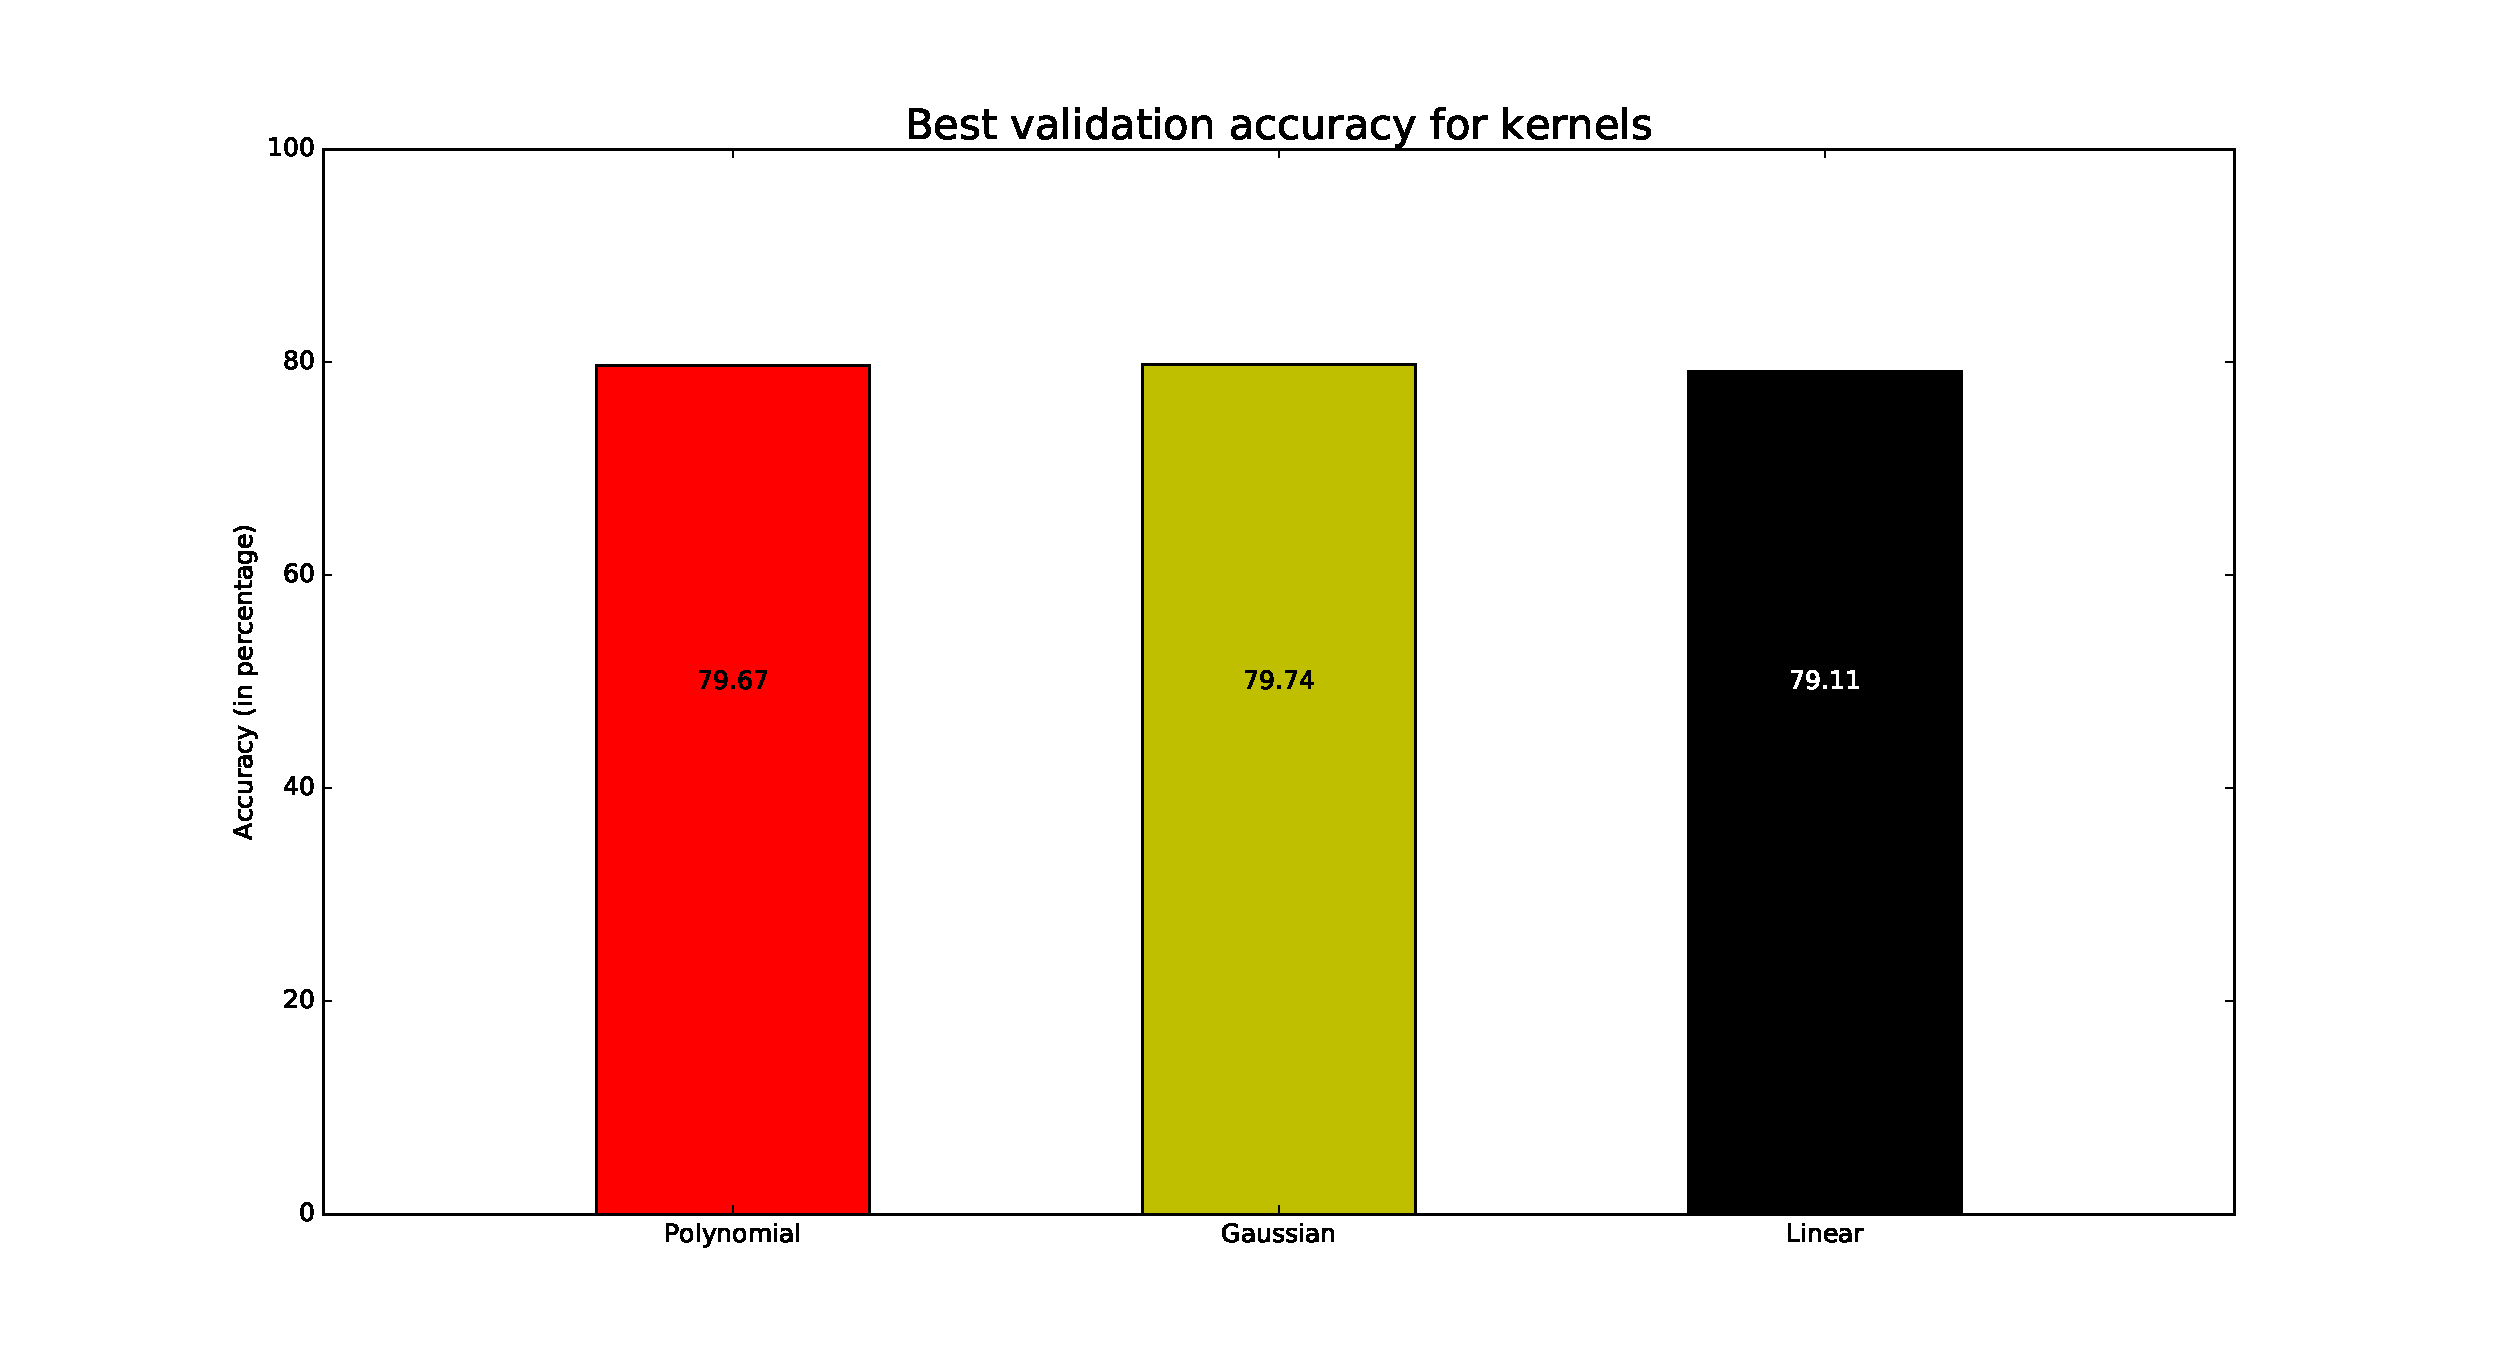
\includegraphics[width=0.5\linewidth]{./images/comparison_3.eps}
\end{figure}

The average time taken to train one cross-validation fold per method is tabulated below:

\begin{center}
\begin{tabular}{|c|c|}
\hline
Method & Time in seconds \\
\hline
\hline
Linear Kernel & \(\approx 75\) \\
\hline
Polynomial Kernel with \(q = 3\) & \(\approx 79\) \\
\hline
Gaussian kernel with \(\sigma = 0.2\) & \(\approx 300\) \\
\hline
\end{tabular}
\end{center}
\end{flushleft}

\section*{Multiple Kernel Learning}
\subsection*{Fixed Rules}
\begin{flushleft}
In Multiple Kernel Learning with fixed rules, it is required to weigh the kernel in a convex combination-fashion. In my study, after infering the results from the single kernel, I chose the following convex combination:
\begin{equation*}
\hat{k} = 0.25*k_{LIN} + 0.35*k_{POL} + 0.4*k_{GAU}
\end{equation*}

The parameters to \(k_{POL}\) and \(k_{GAU}\) remain the same as in the best results for single kernel i.e., \(3\) and \(0.2\) respectively.
\end{flushleft}
\end{document}
